\documentclass[12pt,a4paper]{ctexart}

% ===== 页面设置 =====
\usepackage[top=2.5cm,bottom=2.5cm,left=3cm,right=2.5cm]{geometry}
\usepackage{graphicx,amsmath,amssymb,booktabs,hyperref,caption,enumitem,fancyhdr,float}

% ===== 页眉页脚 =====
\pagestyle{fancy}
\fancyhf{}
\fancyhead[C]{HLA限制型免疫疗法的全球公平性分析}
\fancyfoot[C]{\thepage}
\renewcommand{\headrulewidth}{0.4pt}

% ===== 标题与作者 =====
\title{{\heiti\zihao{2} HLA限制型免疫疗法的全球公平性分析}}
\author{{\kaishu HiChat-fog}\footnote{{\kai GitHub: \url{https://github.com/HiChat-fog}}}}
\date{}

\begin{document}

\maketitle

\begin{center}
{\song\zihao{-4}（中国人民公安大学，北京 102623，China）}
\vspace{0.2cm}

{\song\zihao{-5} GitHub: \url{https://github.com/HiChat-fog/hla-immunotherapy-equity}}
\end{center}

\vspace{0.8cm}

% ===== 摘要（结构化） =====
{\heiti\zihao{4} 摘\ \ 要：}

\vspace{0.3cm}

{\heiti 【目的】}免疫治疗药物Tebentafusp与Afami-cel均依赖HLA-A*02:01呈递肿瘤抗原，而该等位基因在中国胃癌患者中频率仅约5\%，东亚高频的A*11:01（46.9\%）与A*24:02（25.0\%）却无任何对应药物。本研究旨在量化HLA限制型免疫疗法在全球人群中的公平性差距，并提出基于人群HLA分布的靶点优先级优化方案。

{\heiti 【方法】}整合七个独立数据源：GBD全球死因数据（2000--2023年）、GLOBOCAN 2022胃癌负担数据、TCGA-STAD胃癌突变数据（178,508条/393例）、UniProt蛋白序列数据、IEDB MHC-I结合预测数据（2,598条突变肽段x4个HLA等位基因=10,392次预测）、AFND/NMDP/Zhou（2019）HLA人群频率数据及世界银行WDI经济数据。分析管线：非沉默突变筛选→跨突变位点9--11mer肽段提取→IEDB API全矩阵结合预测（percentile rank判定）→贪心覆盖算法优化靶点优先级。

{\heiti 【结果】}A*11:01的强结合新抗原数（27条）为A*02:01（11条）的2.5倍；A*02:01对KRAS的强结合肽段为零条，A*11:01检出5条，A*03:01检出4条。CDH1与SMAD4仅A*24:02有强结合肽段，FBXW7仅A*11:01，ERBB3仅A*03:01。贪心优化后，中国胃癌患者理论覆盖率从FDA现状的5.0\%提升至60.2\%（12.4倍），欧洲仅从26.0\%提升至37.1\%（1.4倍）。HW校正敏感性分析显示优化排序不变，覆盖率稳定于60\%--72\%。A*02:01的SB数（11条）低于随机期望值（约13条，富集倍数0.85倍）。

{\heiti 【局限】}肽-MHC结合预测不等于免疫原性，需体外实验验证；贪心覆盖假设各HLA独立分布，可能存在连锁不平衡偏倚；TCGA-STAD亚洲样本仅87例，存在人群代表性局限。

{\heiti 【结论】}HLA限制型免疫疗法的研发方向存在结构性A*02:01偏好，东亚人群最优靶点A*11:01与A*24:02从未进入研发管线。按贪心覆盖优化重排优先级后，东亚覆盖率可提升12.4倍，公平性差距显著缩小。

\vspace{0.5cm}
{\heiti 关键词：}HLA；免疫治疗；胃癌；新抗原；健康公平性；TCGA-STAD；贪心覆盖优化

\vspace{0.5cm}
{\heiti 中图分类号：}Q811.4 \hspace{1cm} {\heiti 文献标识码：}A

\newpage

% #################### 正文 ####################

\section{引言}

\subsection{研究背景}

免疫治疗正在改变肿瘤治疗的格局。2022年和2024年，Tebentafusp和Afami-cel先后获FDA批准，成为实体瘤TCR-T/CAR-T疗法的里程碑\cite{ref1,ref2}。但两款药物都依赖HLA-A*02:01呈递肿瘤抗原。问题出在HLA的全球分布上——A*02:01在欧洲人群中频率约27\%，在中国胃癌患者中仅约5\%，而A*11:01频率高达47\%，A*24:02达25\%。这两个东亚高频等位基因目前没有任何对应的免疫治疗药物。胃癌东亚负担最重（全球54\%病例），其人群最不可能受益于现有的HLA限制型疗法。这不是医疗资源分配的问题，是基因层面的系统性排斥。

\subsection{研究问题}

本研究回答三个递进问题：（1）HLA频率差异有多大？（2）东亚高频HLA是否真的能有效呈递胃癌新抗原？（3）如果重排研发优先级，能缩小多少公平性差距？

\subsection{技术路线}

分析管线以TCGA-STAD\cite{ref3}的178,508条胃癌突变数据为起点，经UniProt\cite{ref4}蛋白序列提取、跨突变位点肽段生成，通过IEDB API\cite{ref5}完成2,598条独特突变肽段与4个HLA等位基因的全矩阵结合预测（10,392次），预测方法为NetMHCpan-4.1\cite{ref6}。在此基础上用贪心覆盖算法进行靶点优先级优化。

数据层（自下而上）：GBD死因数据\cite{ref7}+GLOBOCAN 2022\cite{ref8}→TCGA-STAD突变数据→UniProt API→IEDB API→AFND\cite{ref10}/NMDP/Zhou等（2019）\cite{ref9}HLA人群频率→世界银行WDI经济协变量。

\newpage

% #################### 2 数据与方法 ####################

\section{数据与方法}

\subsection{数据来源}

本研究整合了七个独立数据源，概况汇总于表1。

\begin{table}[htbp]
\centering
\caption{数据来源汇总}
\label{tab:datasource}
\renewcommand{\arraystretch}{1.1}
\begin{tabular}{lllp{3.5cm}l}
\toprule
数据层 & 来源 & 类型 & 核心字段 & 规模 \\
\midrule
全球死因数据 & GBD & CSV & 国家、年份、死因、死亡人数 & 24文件，203国 \\
胃癌负担 & GLOBOCAN 2022 & 表格 & 国家、癌症部位、ASR & 185国 \\
胃癌突变 & TCGA-STAD（FireBrowse）& MAF & 基因名、突变类型、蛋白改变 & 178,508条 \\
蛋白序列 & UniProt REST API & FASTA & 氨基酸序列 & 约100条 \\
HLA-肽段结合 & IEDB MHC-I API & TSV & allele、peptide、rank、IC50 & 10,392次预测 \\
HLA人群频率 & AFND/NMDP/Zhou 2019 & CSV & allele、population、frequency & 25条记录 \\
经济数据 & 世界银行WDI & CSV & 人均GDP、卫生支出 & 2019--2024 \\
\bottomrule
\end{tabular}
\end{table}

\noindent{\heiti 全球死亡原因数据}来自GBD 2021\cite{ref7}，覆盖203个国家2000--2023年。

\noindent{\heiti 胃癌疾病负担数据}来自GLOBOCAN 2022\cite{ref8}，涵盖185个国家。

\noindent{\heiti 胃癌突变数据}来自TCGA-STAD项目\cite{ref3}，通过FireBrowse API下载，包含178,508条突变记录、393例胃癌样本。核心字段包括Hugo\_Symbol、Variant\_Classification、Protein\_Change（HGVS命名）及SwissProt\_entry\_Id。

\noindent{\heiti 蛋白序列数据}来自UniProt REST API\cite{ref4}，批量获取约100条人类蛋白全长序列。

\noindent{\heiti HLA-肽段结合预测数据}通过IEDB MHC-I Binding Prediction API\cite{ref5}在线获取，共提交2,598条独特突变肽段x4个HLA等位基因=10,392次预测，获得10,333条有效结果。核心字段包括allele、peptide、percentile\_rank和IC50。

\noindent{\heiti HLA人群频率数据}整合三个来源：Allele Frequency Net Database（AFND\cite{ref10}）、NMDP以及Zhou等（2019）\cite{ref9}发表的中国胃癌患者HLA实测分型数据（n=96）。

\noindent{\heiti 经济数据}来自世界银行WDI，包含人均GDP（现价美元）、卫生支出占GDP比例等指标。

\subsection{数据预处理}

原始MAF文件178,508条记录，筛选步骤如下：

（1）过滤同义突变和非编码突变，保留错义突变（Missense\_Mutation），得135,763条。

（2）筛选复发突变。条件：错义突变、有明确蛋白改变标注（p.开头）、有SwissProt ID、在至少2个患者中出现，压缩到约1,640个候选。加策略筛选：取14个已知胃癌驱动基因（TP53、ARID1A、KRAS、PIK3CA、CDH1、ERBB2、RHOA、SMAD4、CTNNB1、APC、PTEN、FBXW7、ERBB3、MET）中的所有突变，再加非驱动基因中出现至少5个患者的突变。

（3）肽段提取。通过UniProt API获取全长蛋白序列，根据蛋白改变标注定位突变位置，提取跨越突变位点的9--11mer肽段。限定9--11mer的原因是HLA-I类肽段结合槽通常容纳8--11个氨基酸，其中9mer和10mer是最主要结合长度。最终得到2,598条独特突变肽段。

HLA频率数据中，中国胃癌患者频率来自Zhou等\cite{ref9}的96例实测分型——这是目前最直接匹配中国胃癌人群的频率参考。

\subsection{新抗原-HLA结合预测方法}

采用IEDB MHC-I Binding Prediction API\cite{ref5}，底层调用NetMHCpan推荐方法\cite{ref6}。以percentile rank而非绝对IC50作为主要判定标准，在每个MHC内部归一化以减少训练集偏差。另加入A*03:01作为中性对照——其欧亚频率均约10--15\%。

结合判定分四档：强结合SB（rank<0.5\%）、弱结合WB（<2.0\%）、边缘结合（<10.0\%）、不结合。SB+WB用于贪心覆盖输入。

工程方面，2,598条肽段x4个HLA=10,392次HTTP请求，实测约需4小时（约19条/分钟）。实现增量保存（每200条结果写一次CSV）和断点续传。最终10,392次预测获得10,333条有效结果，仅59条失败（5.7‰失败率）。

\subsection{互补性与独有性分析}

构建14个驱动基因x4个HLA的SB覆盖矩阵，逐基因检查每个HLA能强结合哪些驱动基因的突变肽段。若A*02:01覆盖的靶点均被其他HLA覆盖，则其在东亚人群中的价值几乎为零；反之，东亚高频HLA若有独有靶点，则这些是目前治疗版图上的盲区。

\subsection{贪心覆盖优化算法}

优化问题描述：有N个药物研发名额，应优先靶向哪些HLA才能在目标人群中覆盖最多患者？

贪心算法逻辑：每次选当前未覆盖人群中频率最高的HLA，纳入优先级列表，更新累积覆盖率，直至饱和。使用等位基因频率而非Hardy-Weinberg校正携带率——有意的保守选择。以HW校正作为敏感性分析验证结论稳健性。

\newpage

% #################### 3 结果 ####################

\section{结果}

\subsection{全球肿瘤负担趋势}

GBD数据显示，全球肿瘤死亡从2000年的703万增长到2023年的1,049万，增幅49.2\%。同期消化系统疾病死亡从204万增至240万，增幅17.8\%——肿瘤的增速接近消化系统疾病的三倍，两者差距从3.4倍扩大到4.4倍。

东亚2023年肿瘤死亡约379万例，绝对负担全球最高；南亚增速最快（+131.7\%）。撒哈拉以南非洲（+124.6\%）和中东北非（+116.6\%）的增速常被忽视——肿瘤负担正从高收入国家向中低收入国家快速转移。人均GDP与肿瘤报告死亡率呈正相关，背后是诊断能力和登记完整性的差异。

GLOBOCAN 2022数据显示，东亚贡献了全球53.8\%的胃癌新发病例，发病率是欧美的5--8倍，胃癌是全球第5高发癌症和第5大癌症死因。

\begin{figure}[htbp]
\centering
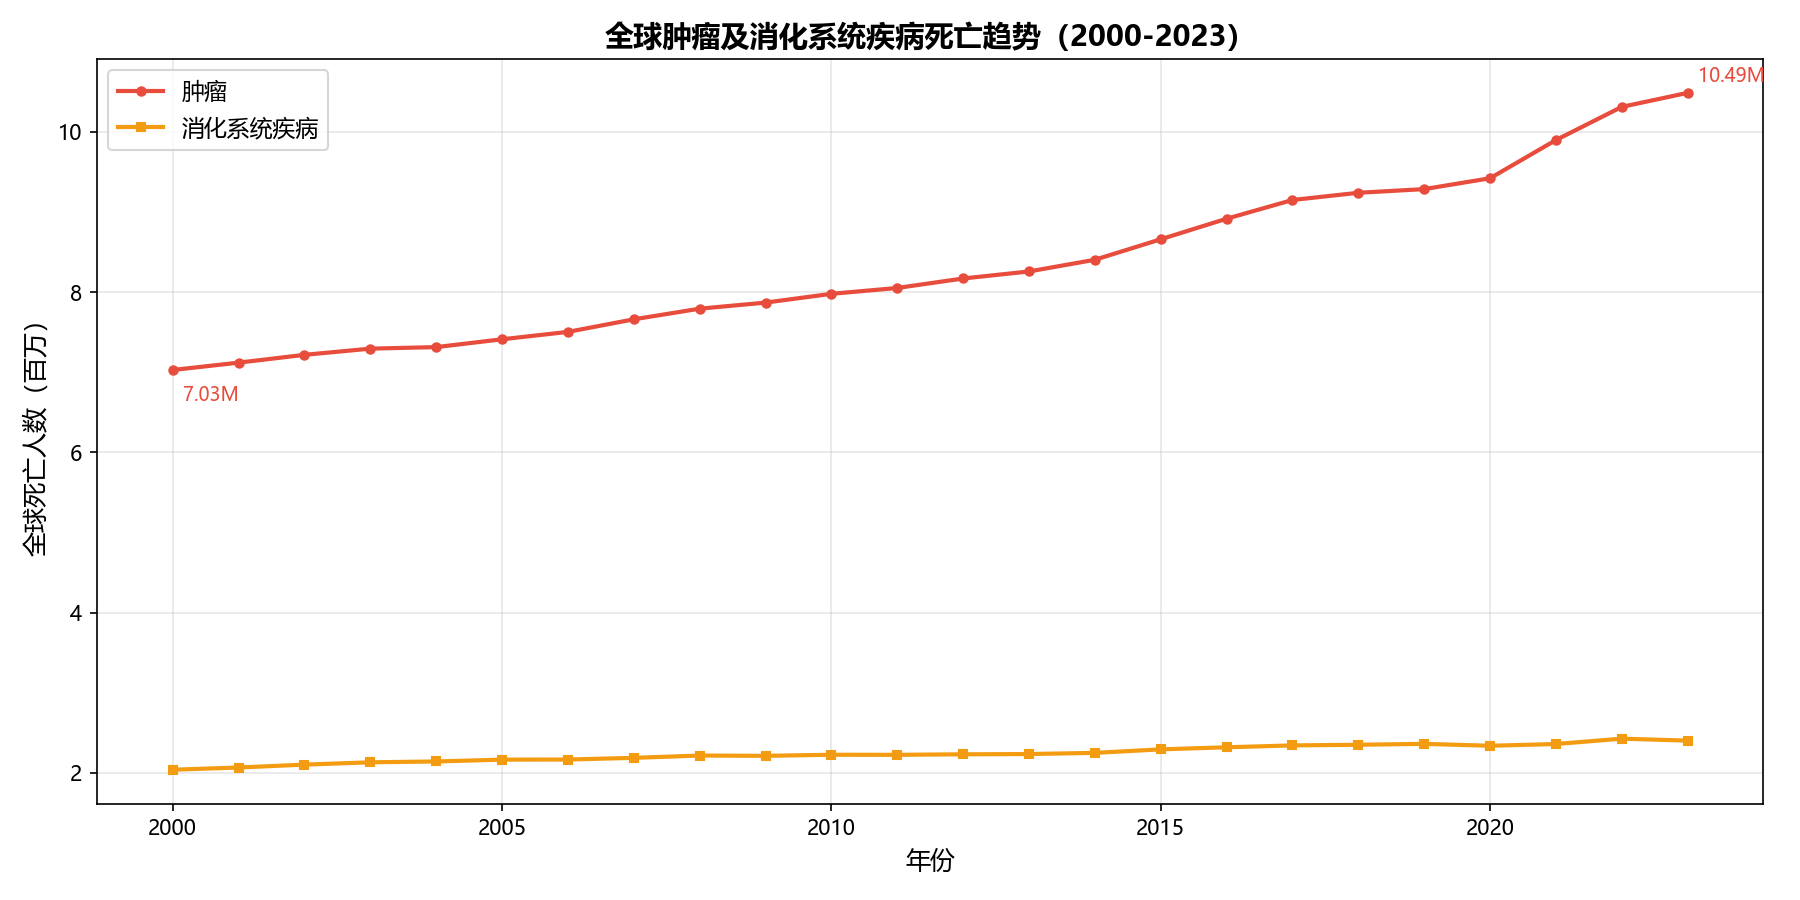
\includegraphics[width=\textwidth]{fig1_global_tumor_trend.png}
\caption{全球肿瘤死亡与消化系统疾病死亡趋势（2000--2023年）}
\label{fig:trend}
\end{figure}

\begin{figure}[htbp]
\centering
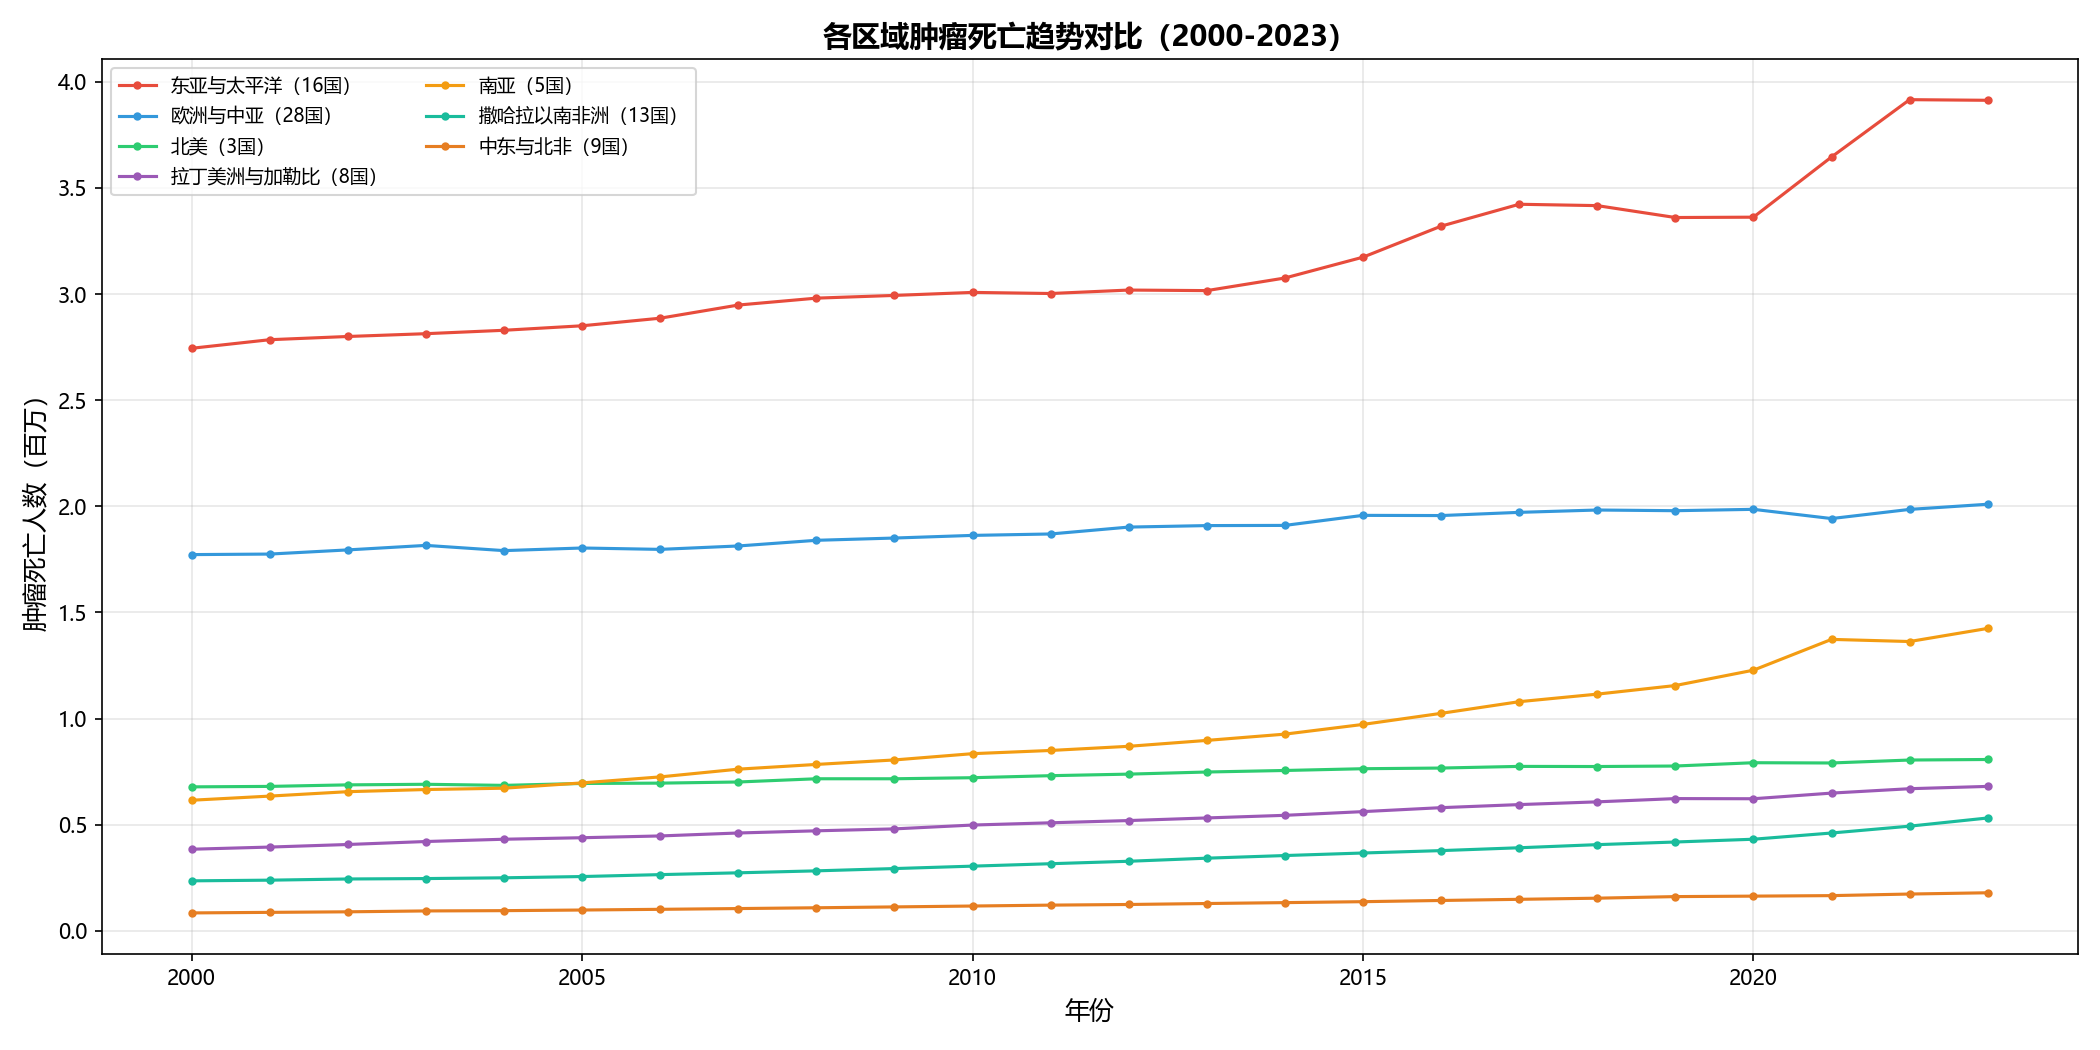
\includegraphics[width=\textwidth]{fig2_regional_tumor_trend.png}
\caption{七区域肿瘤死亡趋势对比}
\label{fig:regional}
\end{figure}

\begin{figure}[htbp]
\centering
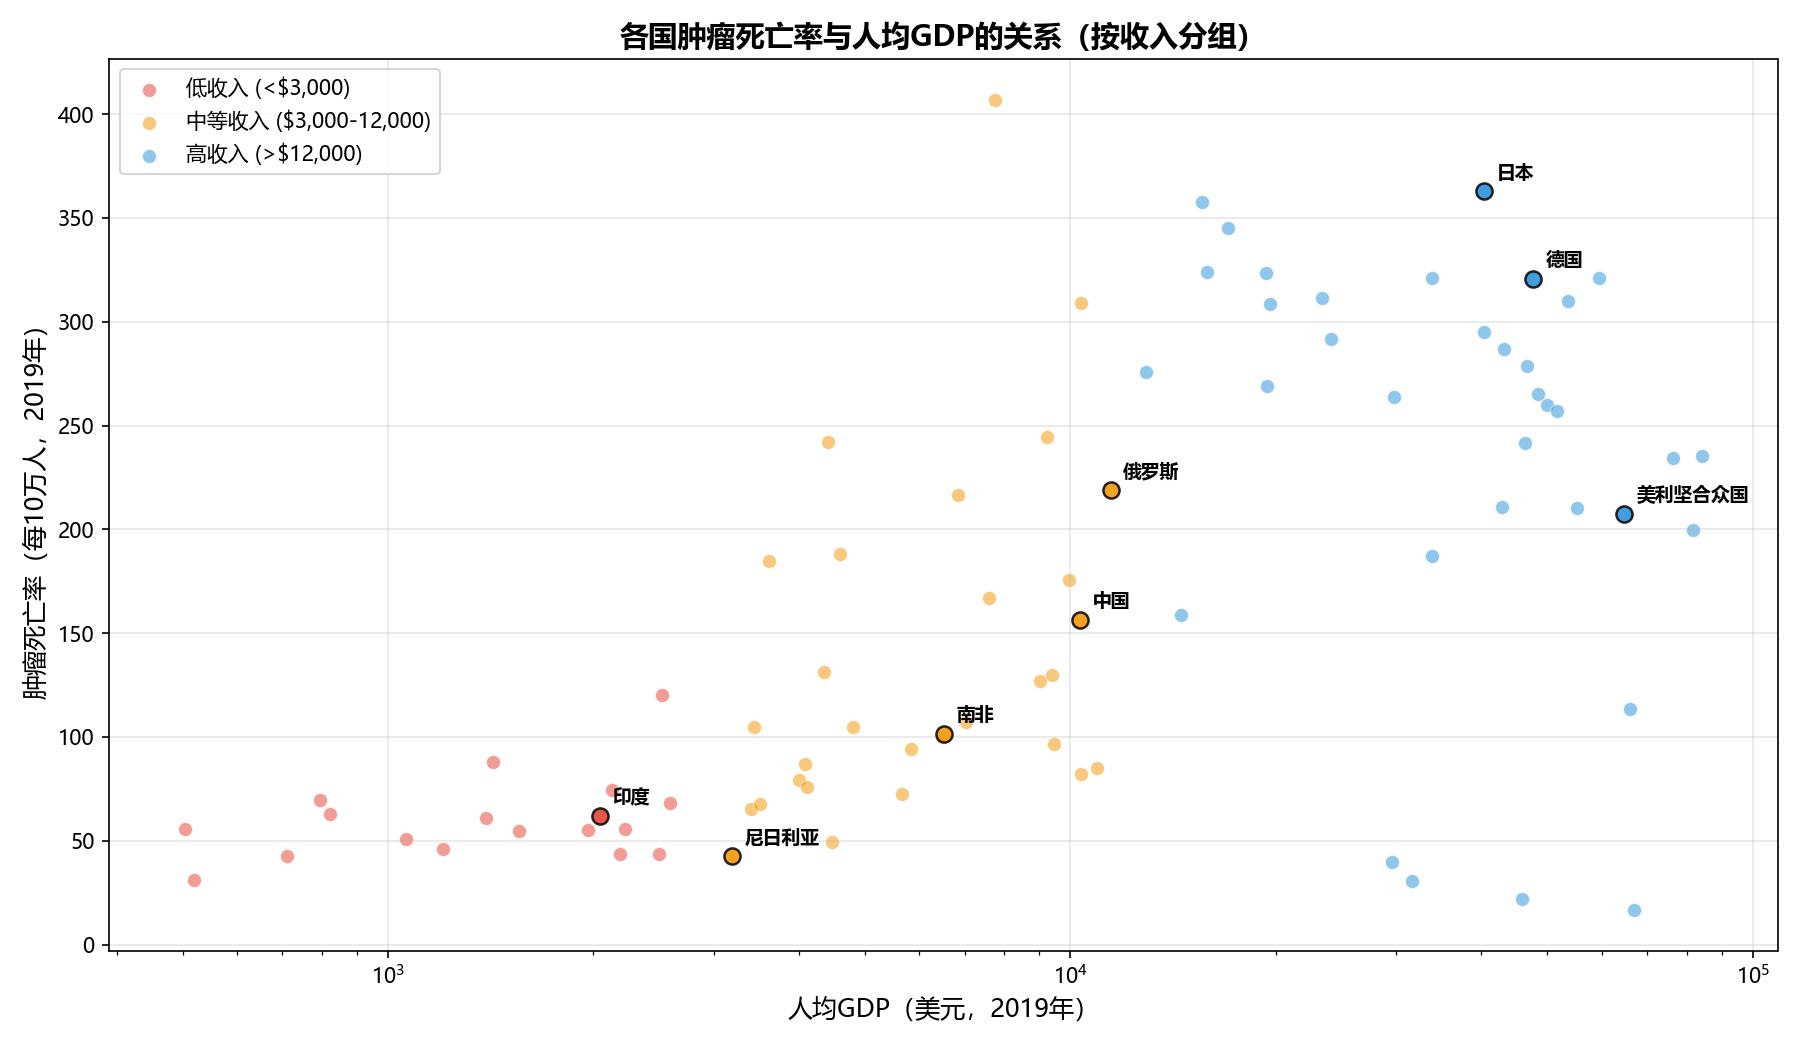
\includegraphics[width=\textwidth]{fig3_income_gdp_vs_tumor.png}
\caption{人均GDP与肿瘤死亡率散点图}
\label{fig:gdp}
\end{figure}

\begin{figure}[htbp]
\centering
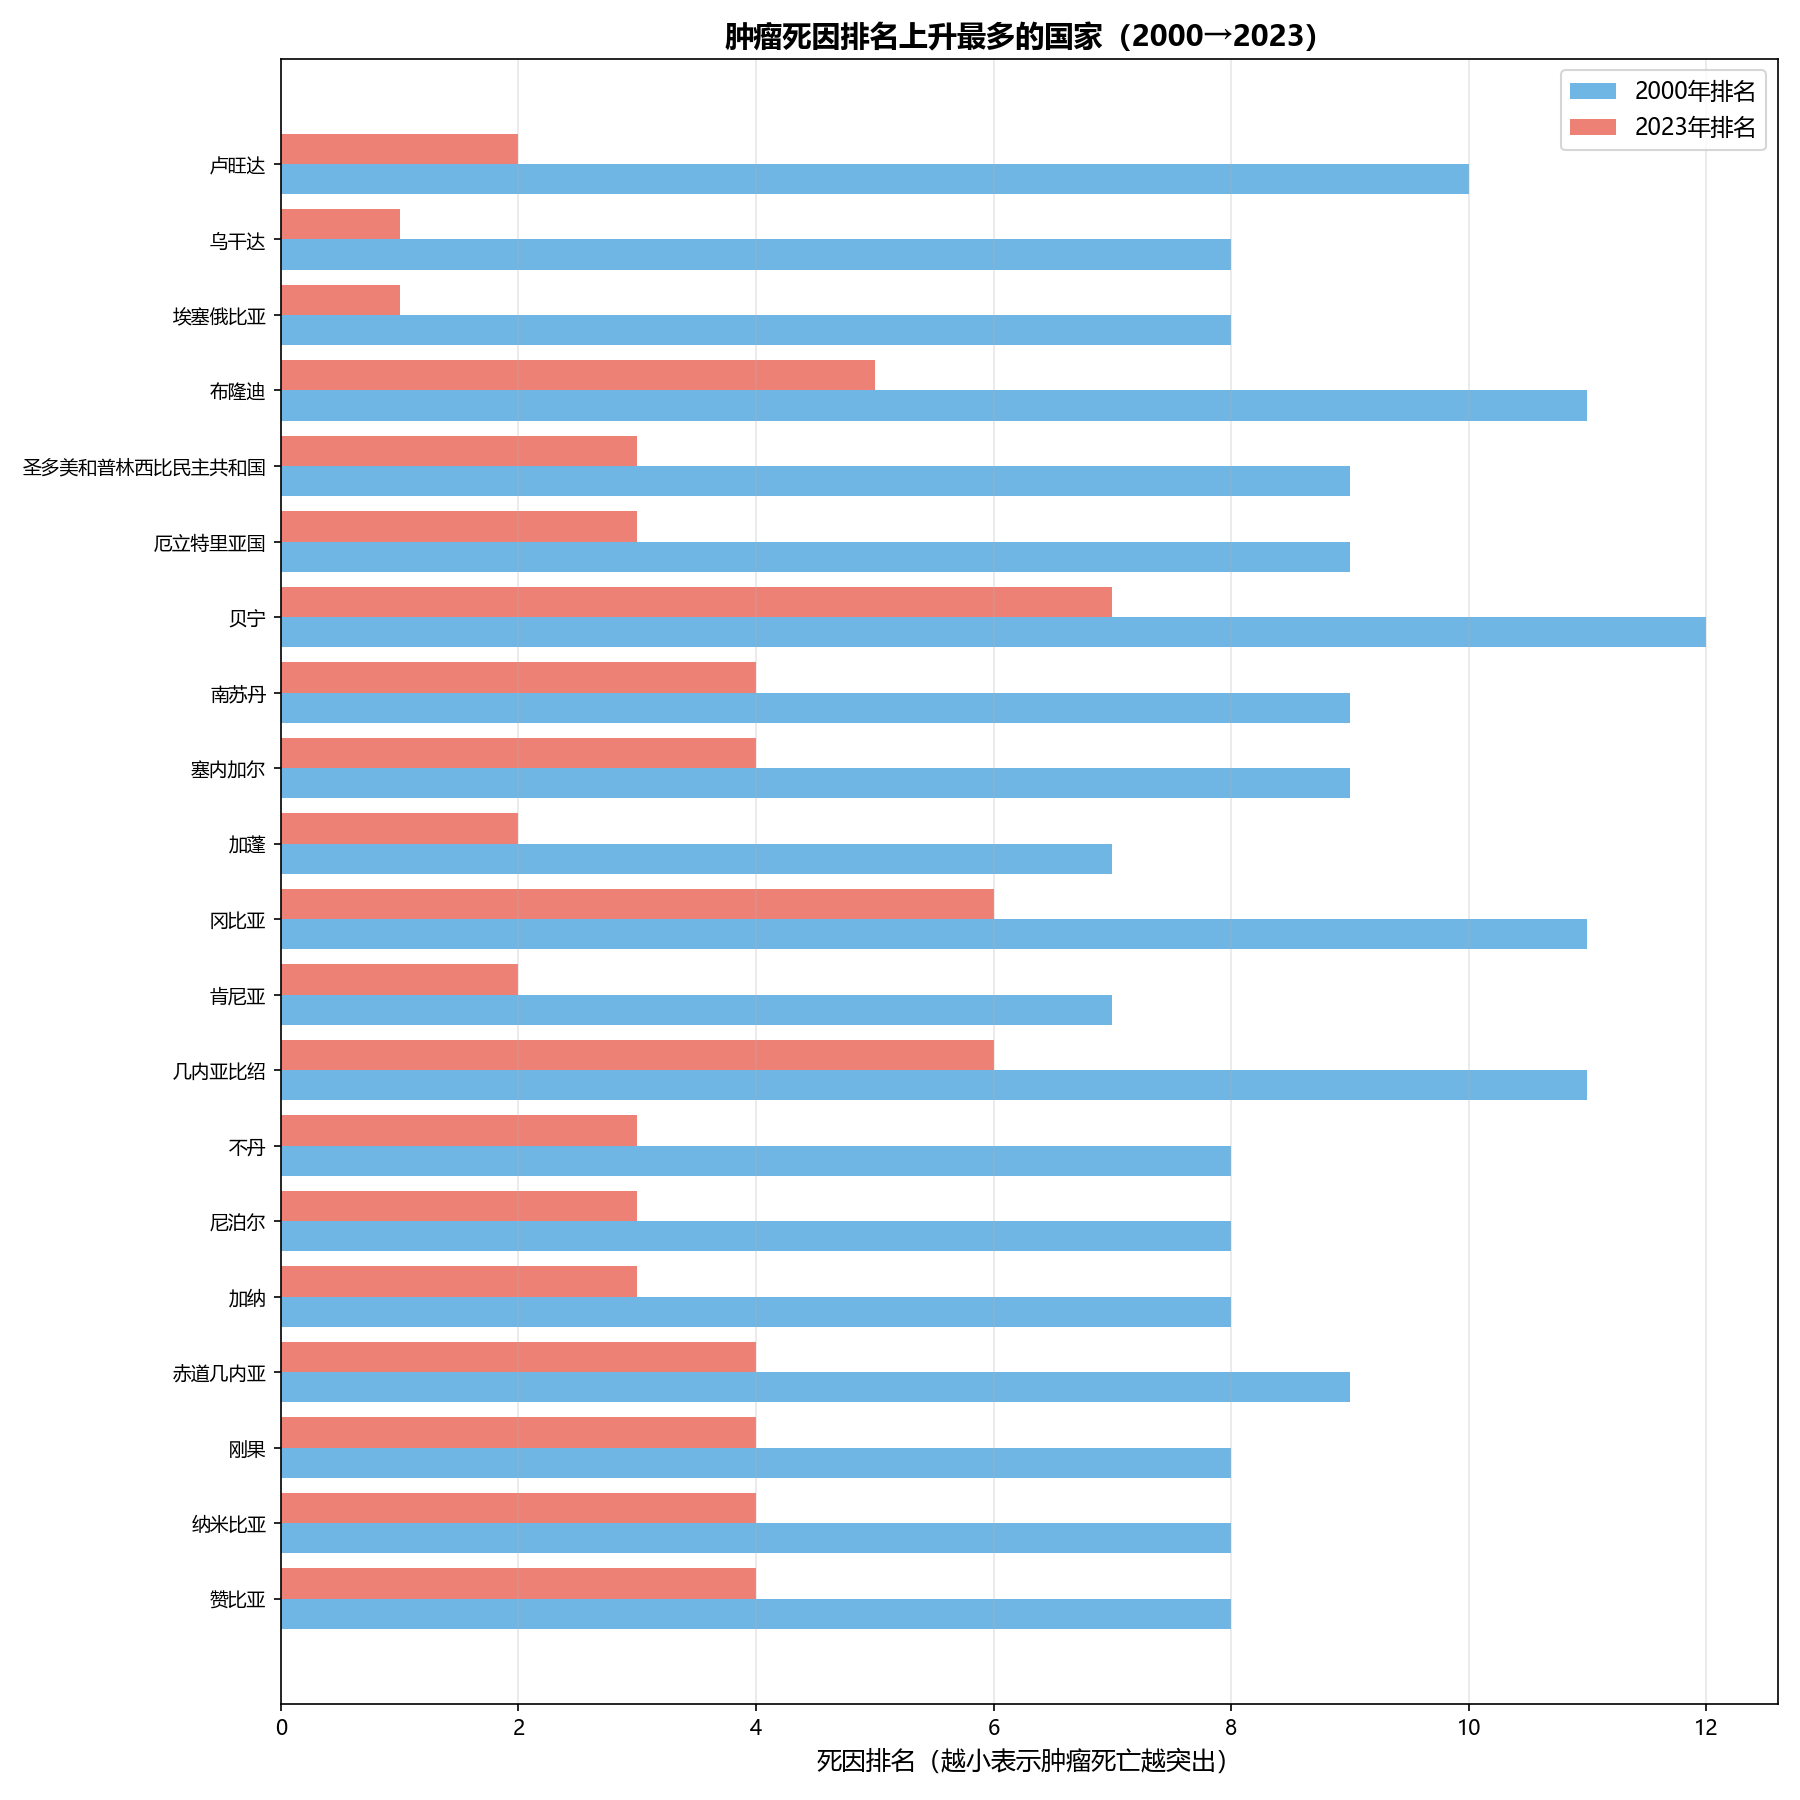
\includegraphics[width=\textwidth]{fig4_tumor_rank_change.png}
\caption{肿瘤在各国死因中的排名变化（2000 vs 2023）}
\label{fig:rank}
\end{figure}

\begin{figure}[htbp]
\centering
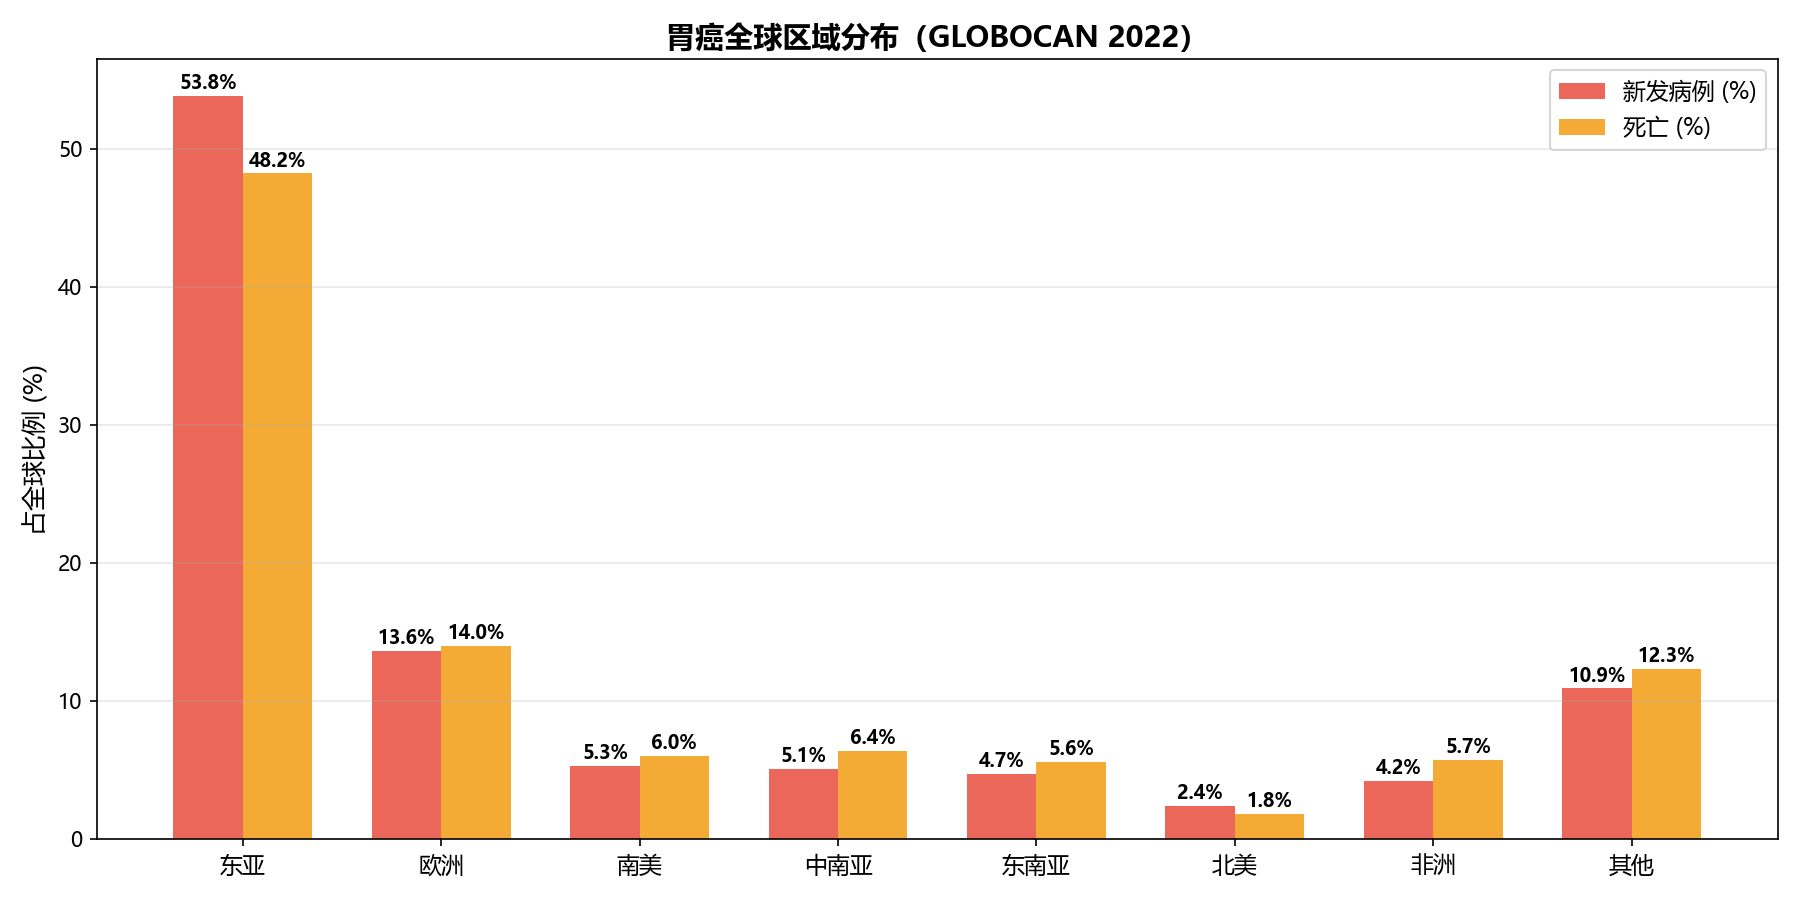
\includegraphics[width=\textwidth]{fig12_global_stomach_cancer.png}
\caption{胃癌全球区域分布（GLOBOCAN 2022）}
\label{fig:globocan}
\end{figure}

\subsection{HLA人群频率差异}

如表\ref{tab:hlafreq}所示，A*02:01在欧洲中位频率26.0\%，在中国胃癌患者中仅5.0\%；A*11:01在中国胃癌患者中46.9\%，欧洲仅5.6\%。A*11:01和A*24:02合计覆盖中国胃癌患者超70\%，对应的免疫治疗药物为零。疾病负担最重的东亚，HLA基因型与现有药物靶点的错配最严重。

\begin{table}[htbp]
\centering
\caption{主要HLA等位基因在东亚与欧洲人群中的频率对比}
\label{tab:hlafreq}
\begin{tabular}{lccc}
\toprule
等位基因 & 中国胃癌患者（Zhou 2019） & 东亚一般人群（NMDP） & 欧洲人群（AFND中位） \\
\midrule
A*02:01 & 5.0\% & 6.5\% & 26.0\% \\
A*11:01 & 46.9\% & — & 5.6\% \\
A*24:02 & 25.0\% & — & 10.0\% \\
\bottomrule
\end{tabular}
\end{table}

\subsection{新抗原-HLA结合预测}

全矩阵预测核心结果汇总于表\ref{tab:hlabind}。A*11:01的SB数（27条）是A*02:01（11条）的2.5倍。A*03:01同样有27条SB——作为中性对照表现强劲，反而加强了论证：问题不在于技术难度，而在于研发方向始终围绕A*02:01。

每个HLA的随机期望假阳性SB约为13条（2,585x0.5\%）。A*02:01的11条低于随机期望（富集倍数0.85x），A*11:01（27条，2.1x）和A*03:01（27条，2.1x）显著高于随机水平——A*02:01对胃癌突变肽段的强结合判定在统计学上无法与随机肽库区分。

\begin{table}[htbp]
\centering
\caption{四个HLA等位基因的胃癌新抗原呈递能力}
\label{tab:hlabind}
\begin{tabular}{lcccc}
\toprule
HLA等位基因 & 强结合SB & 弱+强SB+WB & 覆盖基因(SB+WB) & 覆盖驱动基因(SB) \\
\midrule
A*02:01 & 11 & 62 & 21 & 4 \\
A*11:01 & 27 & 71 & 19 & 6 \\
A*24:02 & 13 & 44 & 15 & 6 \\
A*03:01 & 27 & 67 & 19 & 6 \\
\bottomrule
\end{tabular}

\vspace{0.2cm}
{\small 注：SB: percentile rank<0.5\%; WB: <2.0\%。数据来源：IEDB API全矩阵预测（NetMHCpan-4.1），10,333条有效记录。}
\end{table}

\begin{figure}[htbp]
\centering
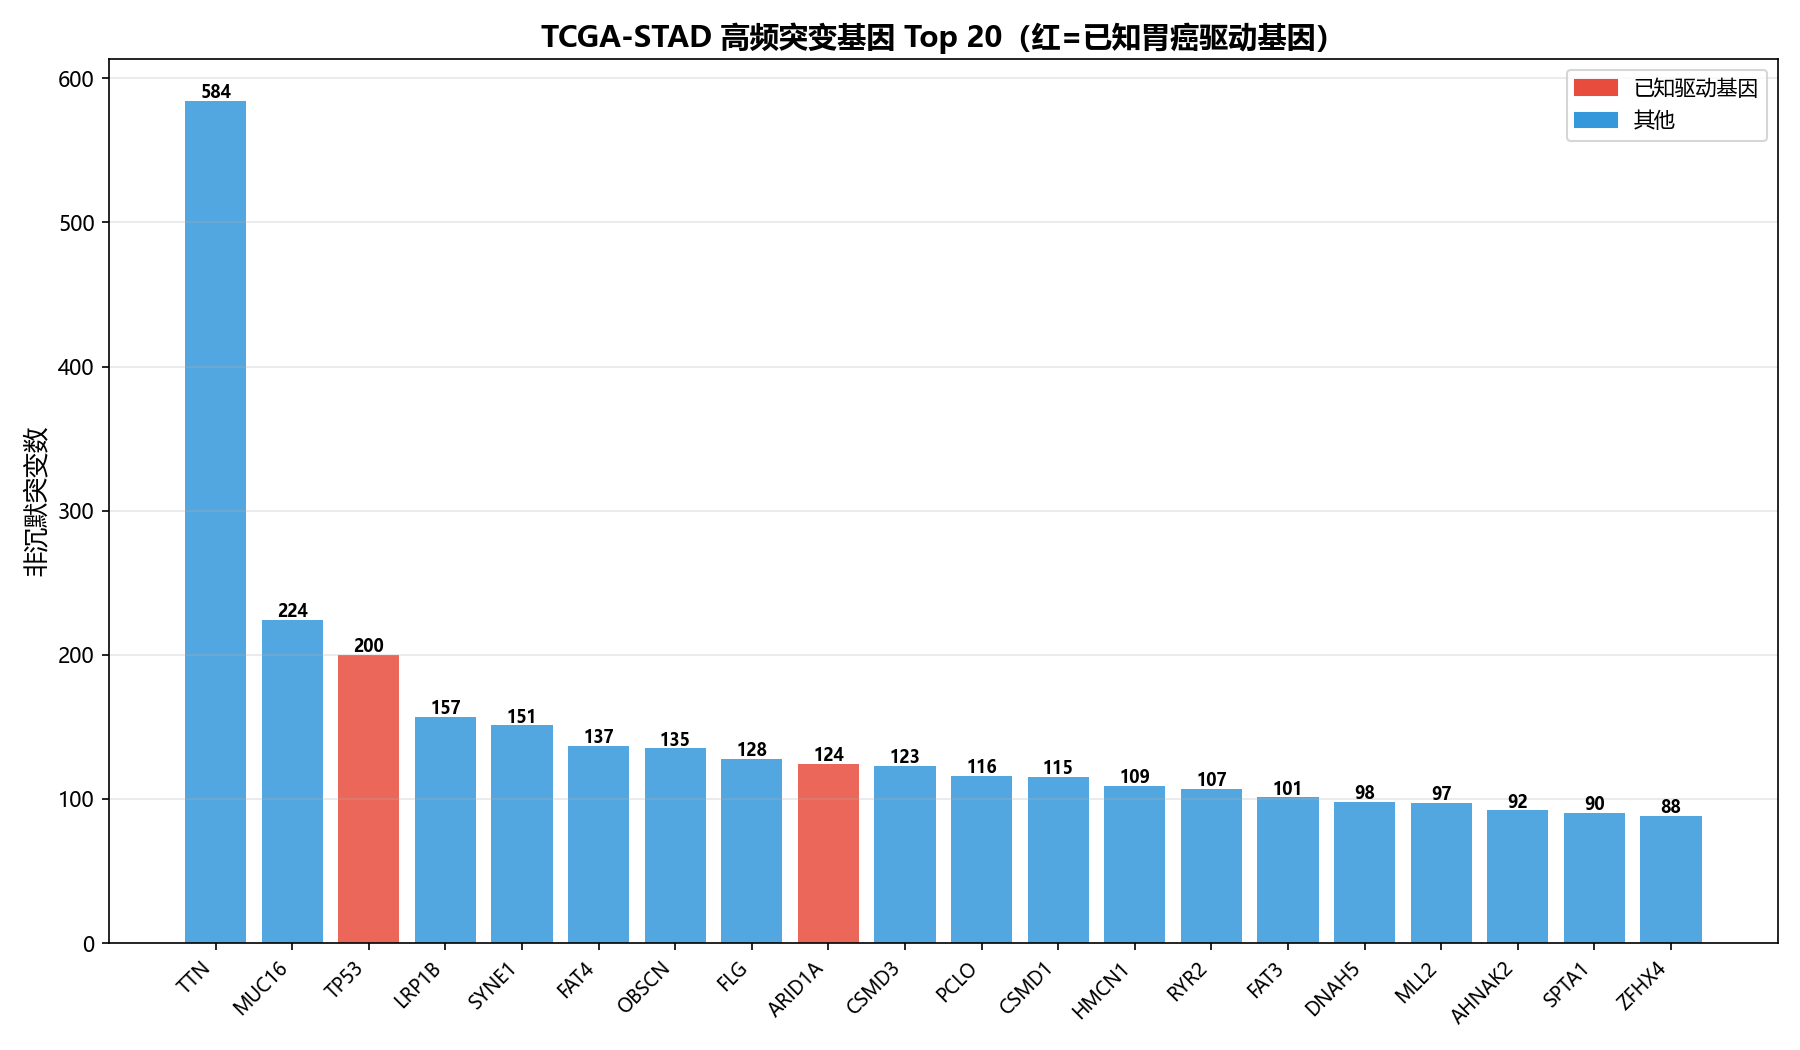
\includegraphics[width=\textwidth]{fig5_top_mutated_genes.png}
\caption{TCGA-STAD高频突变基因（Top 20）}
\label{fig:mutgenes}
\end{figure}

\begin{figure}[htbp]
\centering
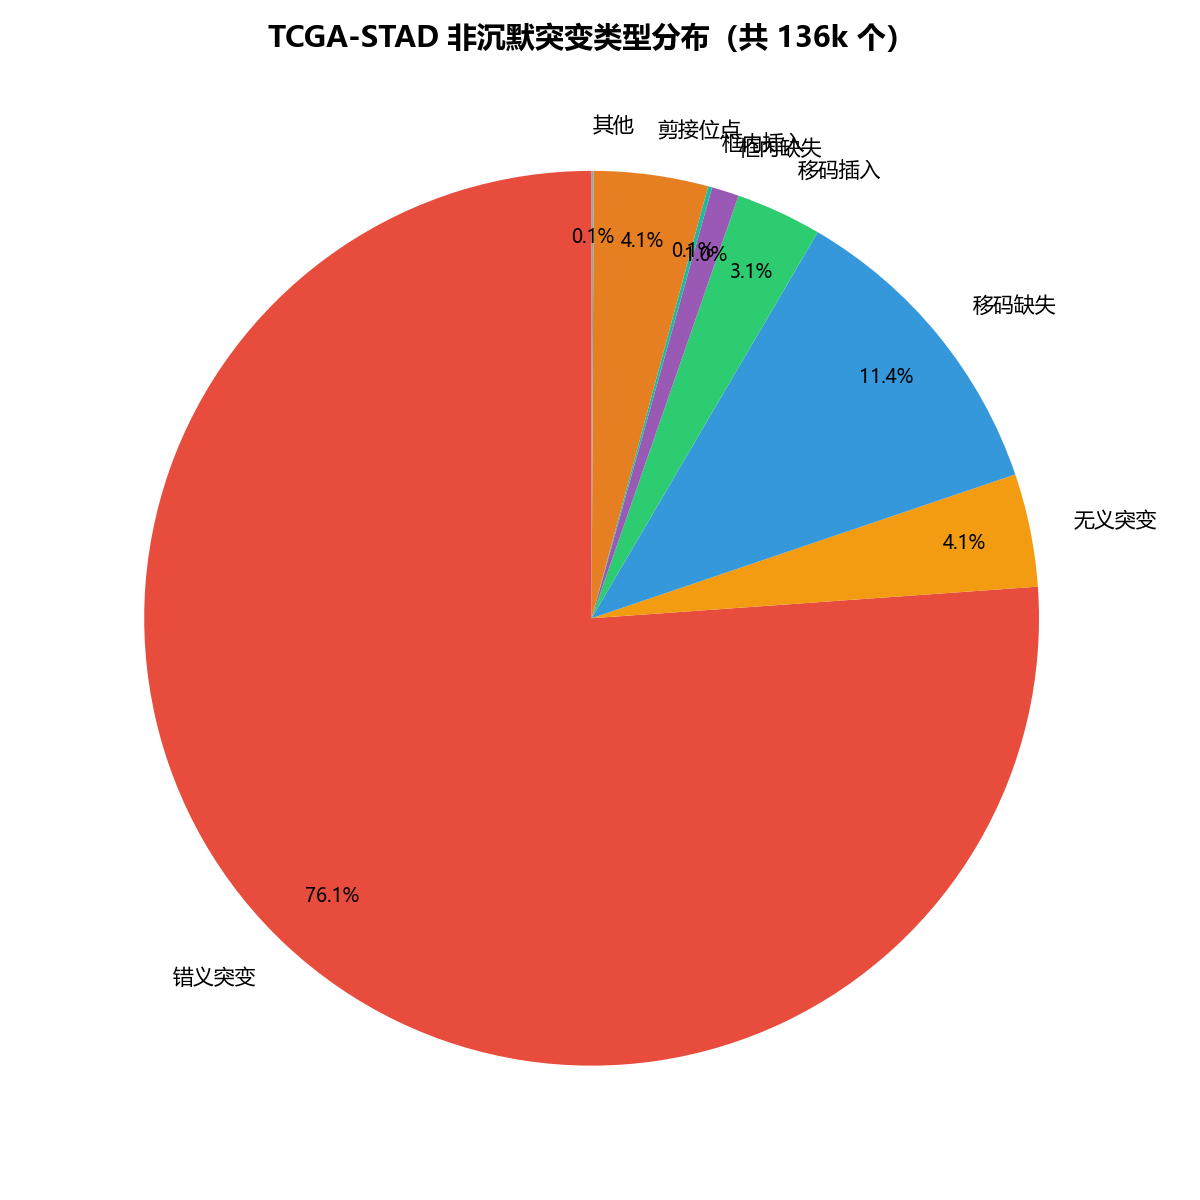
\includegraphics[width=\textwidth]{fig8_mutation_types.png}
\caption{TCGA-STAD非沉默突变类型分布}
\label{fig:muttypes}
\end{figure}

\subsection{驱动基因HLA覆盖互补性}

驱动基因层面的互补性是本分析最关键的发现。覆盖矩阵见表\ref{tab:covermatrix}。

TP53和ERBB2均被四个HLA全覆盖，每个等位基因都有强结合肽段检出。KRAS则明显挑HLA——A*11:01检出5条SB，A*03:01检出4条，A*02:01一条都没有\cite{ref11}。CDH1和SMAD4这两个弥散型胃癌标志基因只在A*24:02里有强结合肽段，FBXW7只在A*11:01，ERBB3只在A*03:01，都是一个HLA单打独斗。A*02:01虽然有4个驱动基因（TP53、PIK3CA、ERBB2、CTNNB1），但这四个基因其他HLA都能覆盖，在东亚人群中并无独占靶点。

\begin{table}[htbp]
\centering
\caption{驱动基因HLA覆盖矩阵（SB层面）}
\label{tab:covermatrix}
\begin{tabular}{lcccc}
\toprule
驱动基因 & A*02:01 & A*11:01 & A*24:02 & A*03:01 \\
\midrule
TP53 & $\checkmark$ & $\checkmark$ & $\checkmark$ & $\checkmark$ \\
PIK3CA & $\checkmark$ & $\checkmark$ & — & $\checkmark$ \\
ERBB2 & $\checkmark$ & $\checkmark$ & $\checkmark$ & $\checkmark$ \\
KRAS & $\times$ & $\checkmark$ & $\times$ & $\checkmark$ \\
CDH1 & — & — & $\checkmark$ & — \\
RHOA & — & $\checkmark$ & $\checkmark$ & $\checkmark$ \\
CTNNB1 & $\checkmark$ & — & $\checkmark$ & — \\
FBXW7 & — & $\checkmark$ & — & — \\
SMAD4 & — & — & $\checkmark$ & — \\
ERBB3 & — & — & — & $\checkmark$ \\
\bottomrule
\end{tabular}

\vspace{0.2cm}
{\small 注：$\checkmark$=该HLA对该基因至少有一条SB肽段；$\times$=已知驱动基因但该HLA无SB；—=未检测到或非该HLA覆盖范围。KRAS的$\times\rightarrow\checkmark\rightarrow\times\rightarrow\checkmark$格局是全文核心论证支点。}
\end{table}

\begin{figure}[htbp]
\centering
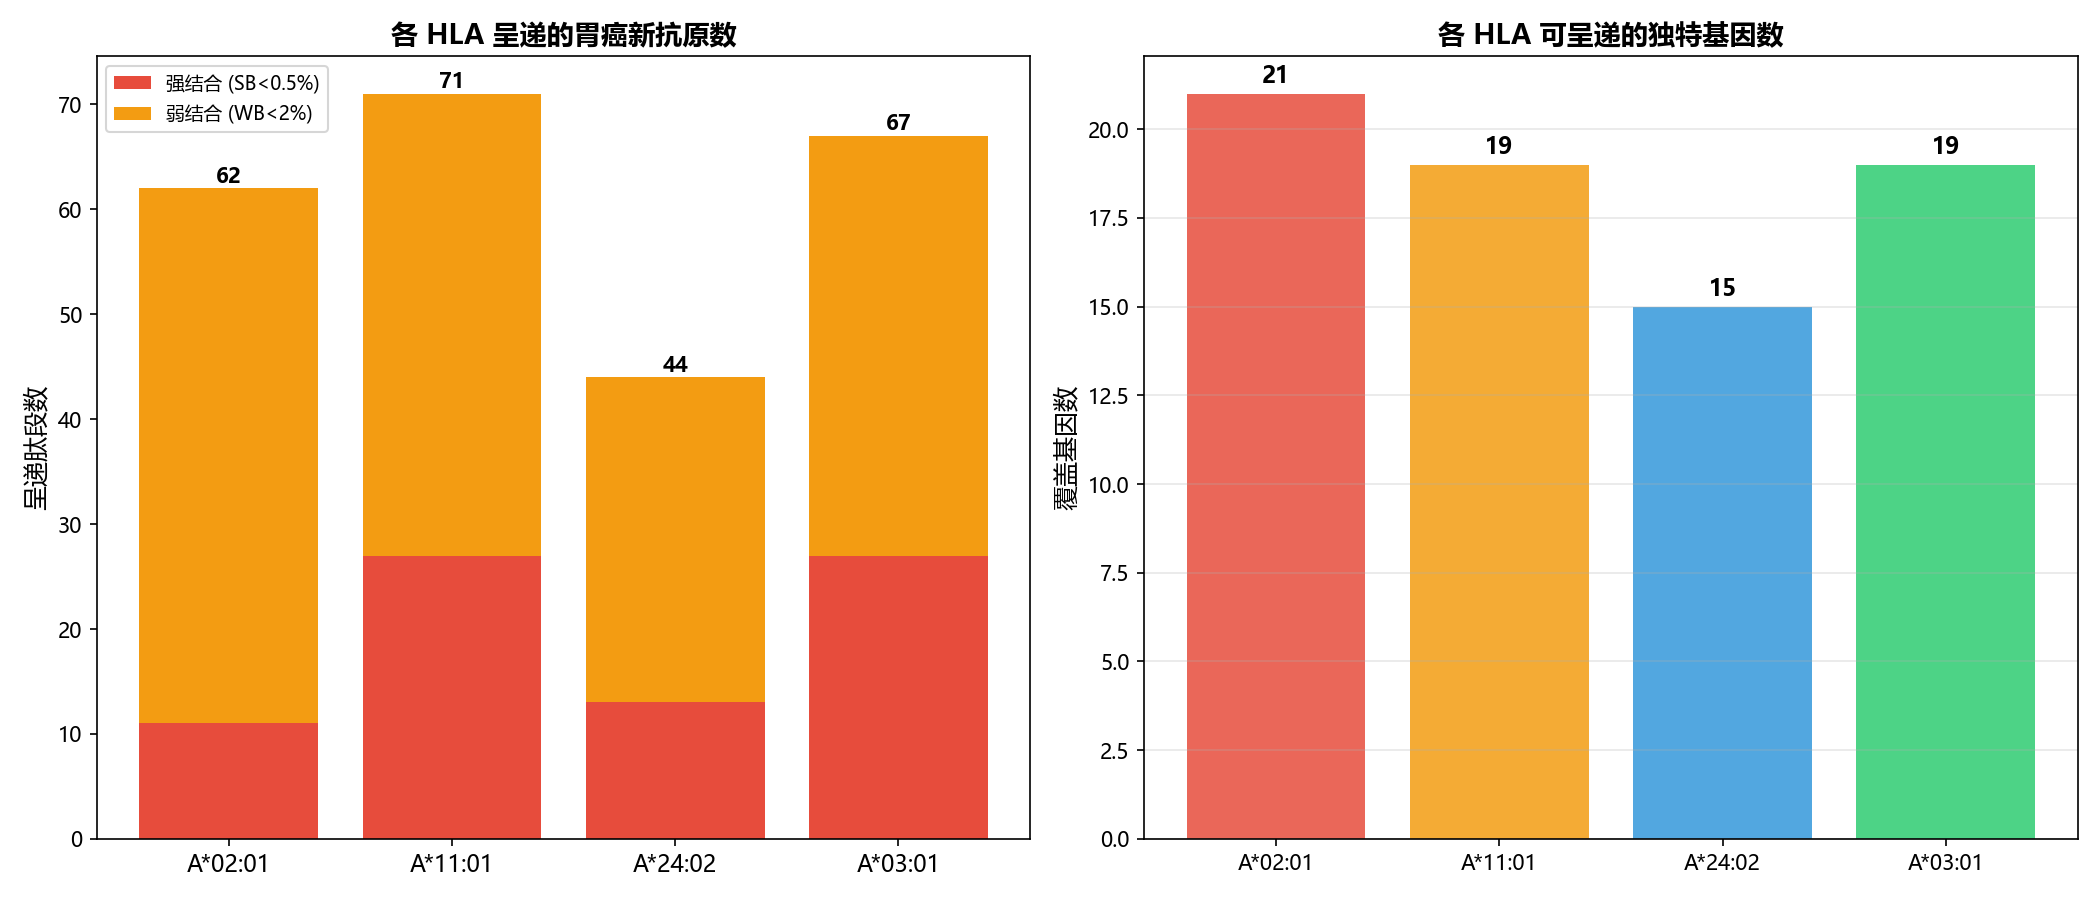
\includegraphics[width=\textwidth]{fig6_hla_presentation_comparison.png}
\caption{四个HLA等位基因的呈递效率对比}
\label{fig:hla_comp}
\end{figure}

\begin{figure}[htbp]
\centering
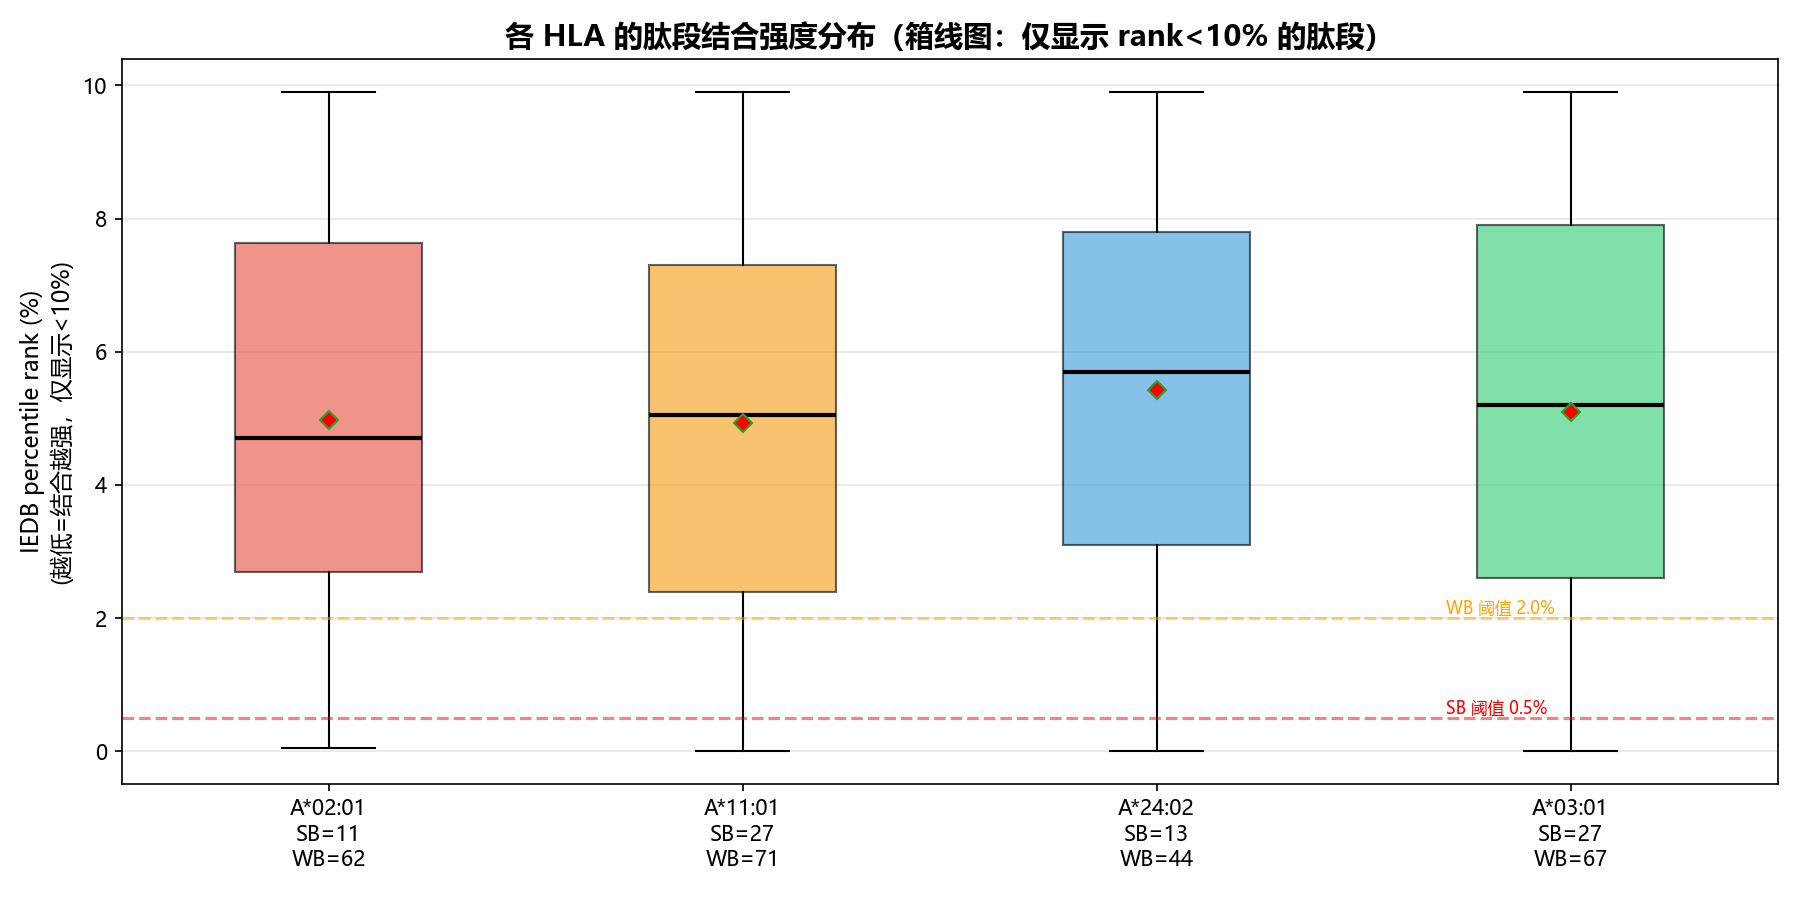
\includegraphics[width=\textwidth]{fig7_rank_distribution.png}
\caption{各HLA的肽段结合强度分布（percentile rank）}
\label{fig:rankdist}
\end{figure}

\begin{figure}[htbp]
\centering
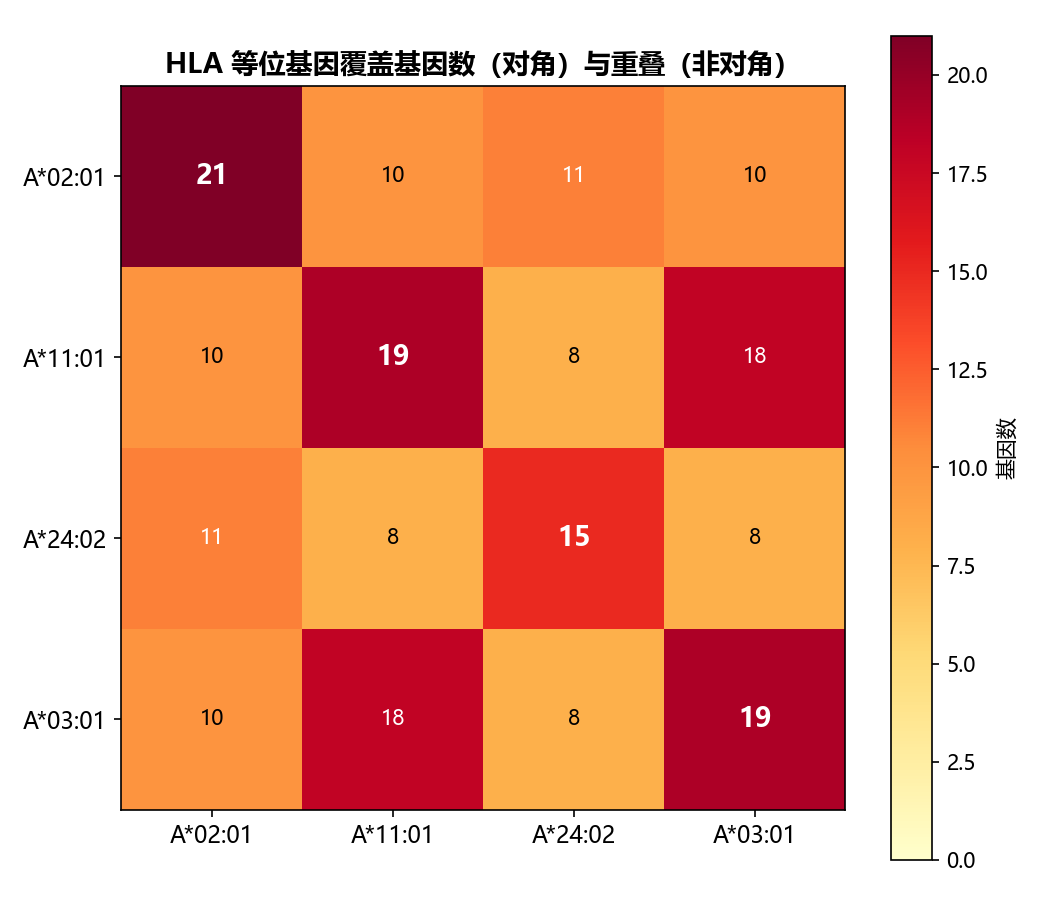
\includegraphics[width=\textwidth]{fig11_gene_overlap_heatmap.png}
\caption{HLA驱动基因覆盖的互补性热力图}
\label{fig:heatmap}
\end{figure}

KRAS值得单独讨论。A*02:01对KRAS突变肽段的强结合数为零——这是结构层面的不匹配，A*02:01的binding motif与KRAS G12D/G12V等关键突变产生的肽段在anchor残基上不对接。A*11:01（5条SB）和A*03:01（4条SB）都能有效呈递。KRAS在胃癌中突变频率8--12\%，预后极差\cite{ref11}，现有HLA限制型疗法对这部分患者完全不适用，这不是数量差距，是有无问题。

\subsection{靶点优先级优化}

贪心覆盖优化结果见表\ref{tab:greedy}。中国队列从A*11:01起步（46.9\%），加A*24:02后累计60.2\%，第三步加A*02:01仅涨2\%，边际增益很有限。欧洲队列的曲线平坦得多——从A*02:01起步26.0\%，每一步提升都不到10\%。

\begin{table}[htbp]
\centering
\caption{贪心覆盖优化结果}
\label{tab:greedy}
\begin{tabular}{llcll}
\toprule
优先级 & 中国—等位基因 & 累积覆盖率（中国） & 欧洲—等位基因 & 累积覆盖率（欧洲） \\
\midrule
FDA现状 & A*02:01 & {\heiti 5.0\%} & A*02:01 & {\heiti 26.0\%} \\
第1优先 & A*11:01 & 46.9\% & A*24:02 & 33.4\% \\
第2优先 & A*24:02 & {\heiti 60.2\%} & A*11:01 & {\heiti 37.1\%} \\
第3优先 & A*02:01 & 62.2\% & — & — \\
\bottomrule
\end{tabular}

\vspace{0.2cm}
{\small 注：使用原始等位基因频率，非HW校正携带率。数据来源：HLA频率（Zhou 2019\cite{ref9}/AFND\cite{ref10}）x贪心覆盖算法。}
\end{table}

中国患者从5.0\%提升到优化方案的60.2\%，翻了12.4倍。欧洲从26.0\%到37.1\%，只有1.4倍。这个差距不是研发水平的差距，单纯是运气问题——A*02:01恰好是欧洲人群的最优靶点，FDA的研发路线天然匹配了西方人群。而东亚的最优靶点A*11:01和A*24:02从来没进过研发管线\cite{ref12,ref13}。

用HW校正携带率（A*11:01=71.8\%）做敏感性分析，优化排序不变，覆盖率落在60\%--72\%之间，结论对方法学假设不敏感。

\begin{figure}[htbp]
\centering
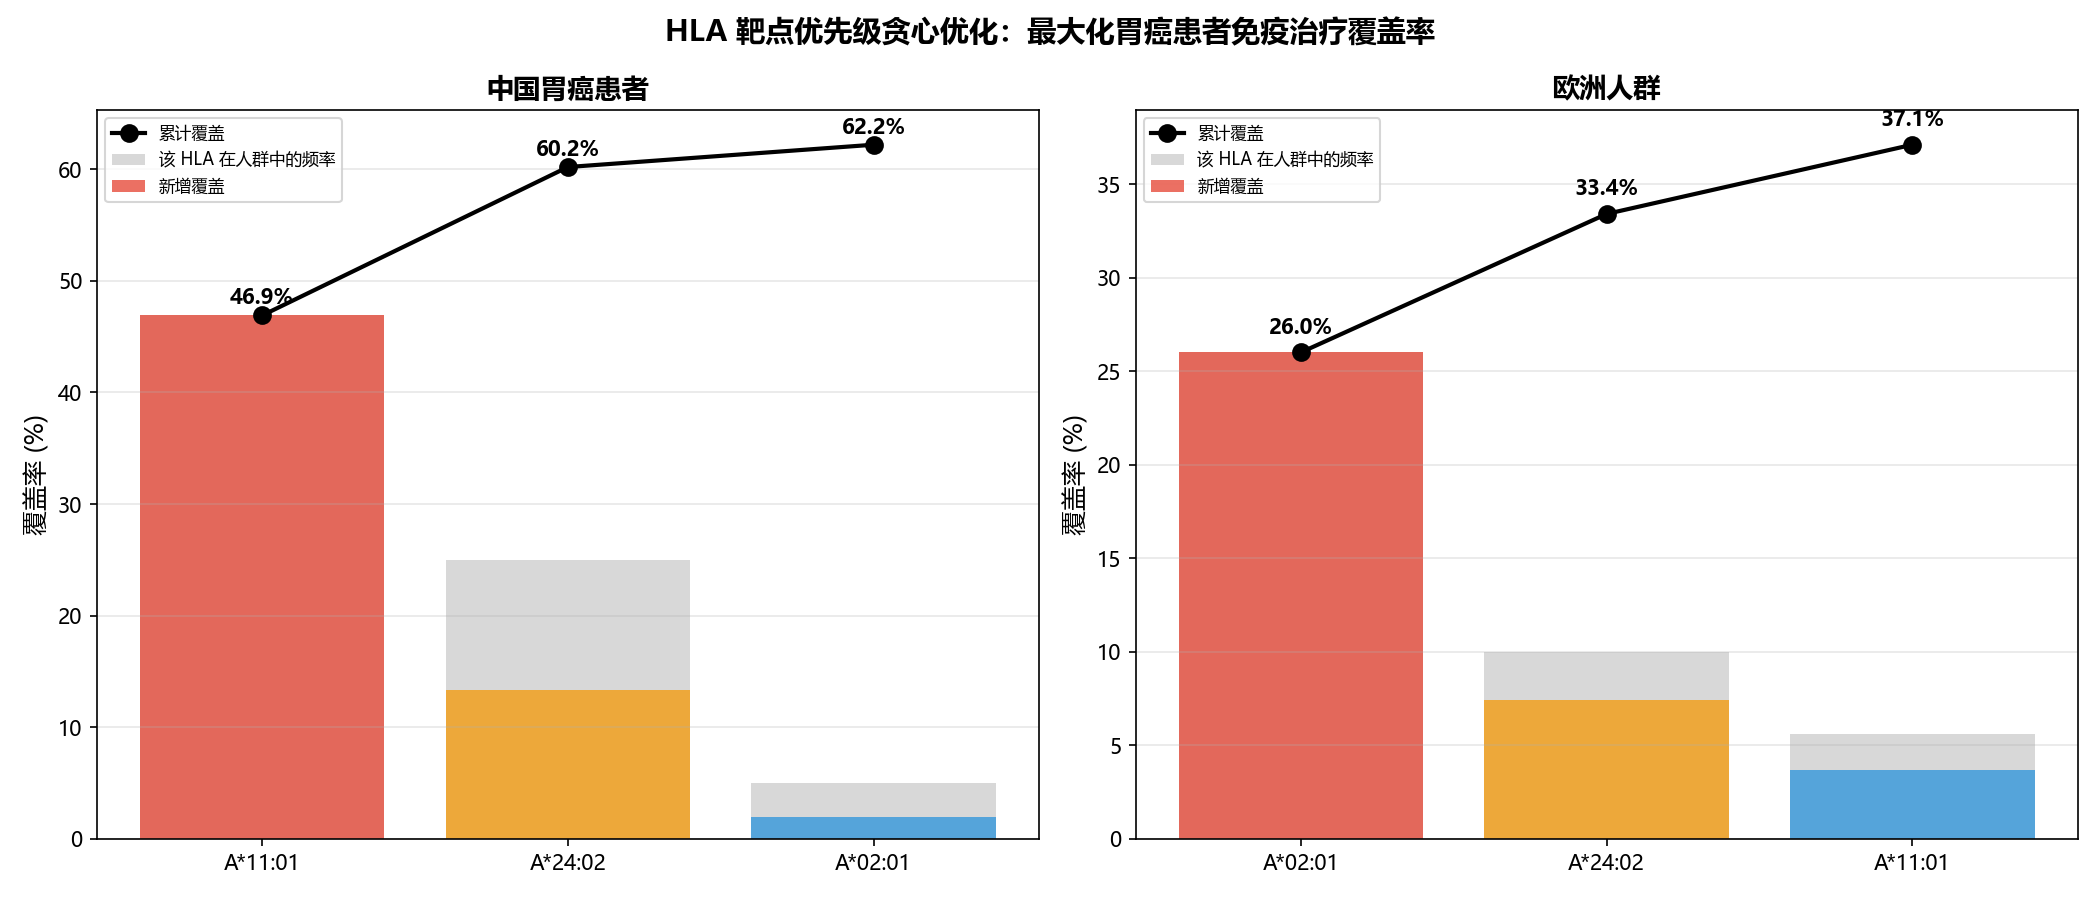
\includegraphics[width=\textwidth]{fig9_greedy_coverage.png}
\caption{贪心覆盖累积曲线——中国 vs 欧洲}
\label{fig:greedy}
\end{figure}

\begin{figure}[htbp]
\centering
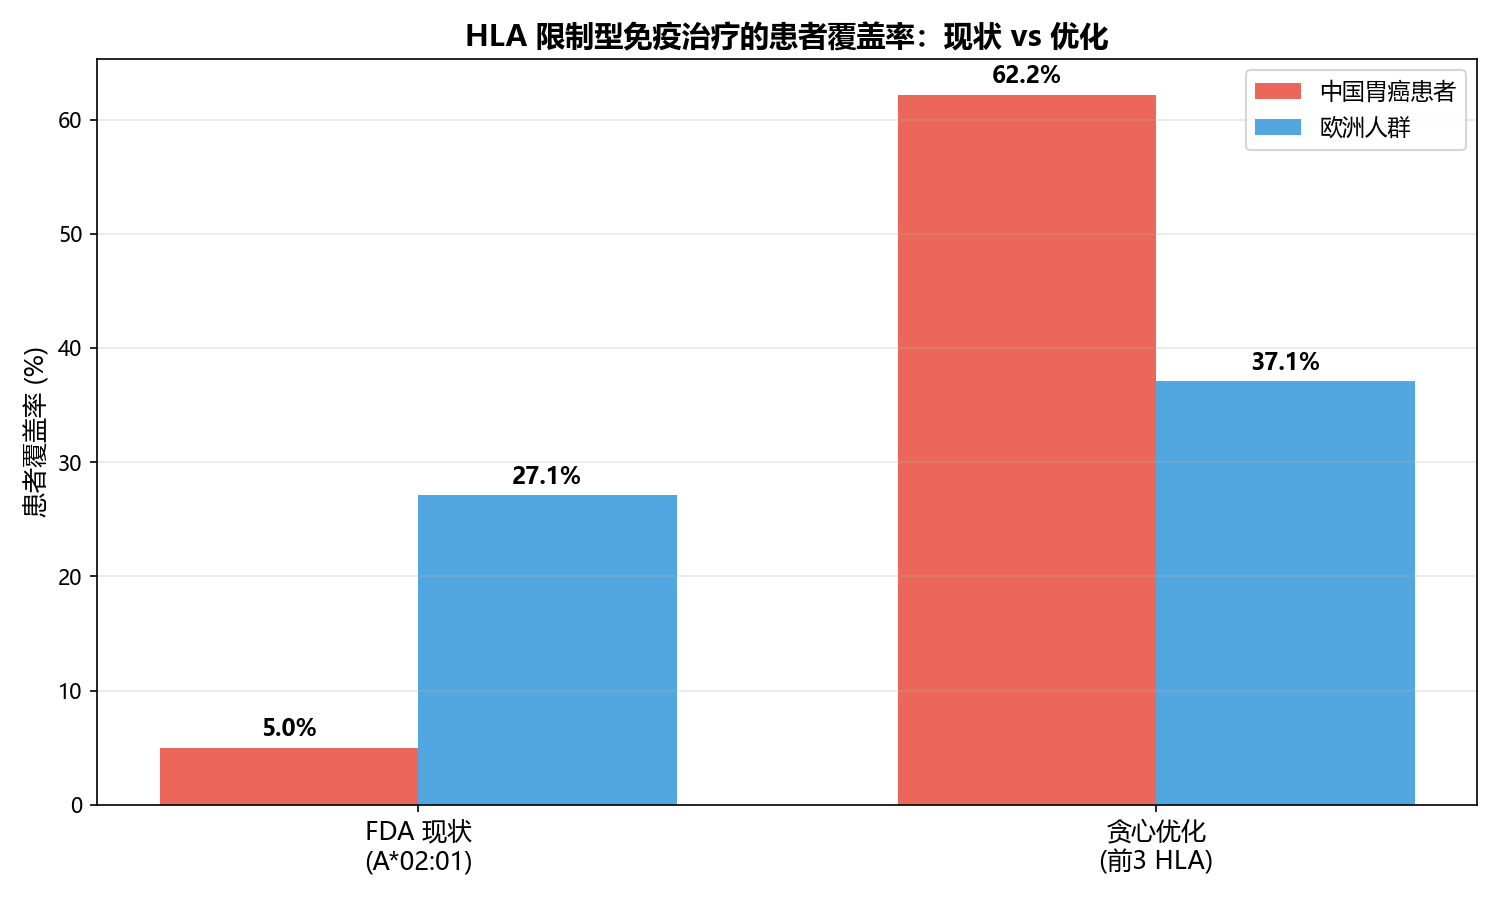
\includegraphics[width=\textwidth]{fig10_coverage_comparison.png}
\caption{FDA现状 vs 优化方案的覆盖率对比}
\label{fig:fdacomp}
\end{figure}

\newpage

% #################### 4 讨论 ####################

\section{讨论}

\subsection{公平性差距的结构性成因}

本研究发现HLA限制型免疫疗法的公平性差距并非偶然。A*02:01恰好是欧洲人群的最优靶点，FDA的研发路线天然匹配西方人群。而东亚的最优靶点A*11:01和A*24:02从未进入研发管线。这种结构性偏差与Smithy等\cite{ref12}和Oseni等\cite{ref13}提出的HLA异质性驱动型癌症健康差异（HACHD）概念一致——当前治疗策略在未意识到的情况下加剧了健康不平等。

\subsection{KRAS的泛癌种推广}

KRAS G12D/G12V/G12C是泛癌种驱动突变——胰腺癌中约90\%，结直肠癌约40\%，肺腺癌约30\%。胃癌反而是这几个癌种中KRAS频率偏低的（约8--12\%）。本研究的发现提供了lower bound估计：在KRAS突变频率最低的癌种中已经存在显著公平性差距，推广到其他癌种只会更严重\cite{ref11}。A*11:01和A*24:02联合覆盖约60\%中国患者，对药企靶点选择有直接参考价值。

\subsection{局限性}

（1）肽-MHC结合预测不等于免疫原性。肽段能稳定结合HLA是T细胞识别的必要条件，不是充分条件——还需要存在能识别该pMHC复合物的T细胞克隆\cite{ref14,ref15}。本研究的定位是必要条件论证：如果连结合都做不到（如A*02:01对KRAS），后续T细胞识别就不需要讨论了。

（2）贪心覆盖假设各HLA独立分布，A*11:01和A*24:02同处HLA-A基因座时存在系统性偏差，经HW校正敏感性分析验证排序不变，结论方向稳健。

（3）TCGA-STAD中亚洲样本仅87例\cite{ref3}——这是TCGA本身的代表性局限。但核心结论不依赖TCGA的亚洲样本量：HLA频率来自独立中国人群队列\cite{ref9}，驱动基因验证有独立文献支持，预测对象是公共突变（高频复发）而非个体私有突变。

\subsection{后续方向}

（1）扩展至HLA-B和HLA-C基因座，本研究4个等位基因仅为起点；\\
（2）用更大规模亚洲胃癌基因组数据补充TCGA的代表性不足；\\
（3）对A*11:01预测最强的若干肽段做体外结合验证；\\
（4）将分析框架推广至其他HLA限制型疗法适应症（如胰腺癌、结直肠癌）。

\newpage

% #################### 5 结论 ####################

\section{结论}

本研究通过整合TCGA-STAD突变数据、IEDB全矩阵结合预测和贪心覆盖优化，对HLA限制型免疫疗法的全球公平性进行了系统性量化分析。主要发现：

（1）A*11:01的胃癌新抗原呈递能力（27条SB）为A*02:01（11条）的2.5倍，且独有KRAS和FBXW7的呈递能力。

（2）A*02:01对KRAS的强结合肽段为零，对胃癌突变肽段的强结合判定在统计学上无法与随机肽库区分（富集倍数0.85x）。

（3）贪心优化后，中国胃癌患者理论覆盖率从5.0\%提升至60.2\%（12.4倍），欧洲仅从26.0\%提升至37.1\%（1.4倍）。差距根源在于研发方向的结构性A*02:01偏好。

（4）HW校正敏感性分析验证结论稳健（覆盖率60\%--72\%，排序不变）。

综上，HLA限制型免疫疗法的研发方向存在结构性A*02:01偏好，按人群HLA分布重排研发优先级可显著缩小公平性差距，尤其对胃癌负担最重的东亚人群。

\newpage

% #################### 参考文献 ####################

\begin{thebibliography}{15}

\bibitem{ref1} Nathan P, Hassel J C, Rutkowski P, et al. Overall survival benefit with tebentafusp in metastatic uveal melanoma[J]. New England Journal of Medicine, 2021, 385(13): 1196-1206.

\bibitem{ref2} D'Angelo S P, Araujo D M, Abdul Razak A R, et al. Afamitresgene autoleucel for advanced synovial sarcoma and myxoid round cell liposarcoma (SPEARHEAD-1): an international, open-label, phase 2 trial[J]. The Lancet, 2024, 403(10435): 1460-1471.

\bibitem{ref3} Cancer Genome Atlas Research Network. Comprehensive molecular characterization of gastric adenocarcinoma[J]. Nature, 2014, 513(7517): 202-209.

\bibitem{ref4} UniProt Consortium. UniProt: the universal protein knowledgebase in 2023[J]. Nucleic Acids Research, 2023, 51(D1): D523-D531.

\bibitem{ref5} Vita R, Mahajan S, Overton J A, et al. The Immune Epitope Database (IEDB): 2018 update[J]. Nucleic Acids Research, 2019, 47(D1): D339-D343.

\bibitem{ref6} Reynisson B, Alvarez B, Paul S, et al. NetMHCpan-4.1 and NetMHCIIpan-4.0: improved predictions of MHC antigen presentation by concurrent motif deconvolution and integration of MS MHC eluted ligand data[J]. Nucleic Acids Research, 2020, 48(W1): W449-W454.

\bibitem{ref7} GBD 2021 Causes of Death Collaborators. Global burden of 288 causes of death and life expectancy decomposition in 204 countries and territories and 811 subnational locations, 1990-2021[J]. The Lancet, 2024, 403(10440): 2100-2132.

\bibitem{ref8} Bray F, Laversanne M, Sung H, et al. Global cancer statistics 2022: GLOBOCAN estimates of incidence and mortality worldwide for 36 cancers in 185 countries[J]. CA: A Cancer Journal for Clinicians, 2024, 74(3): 229-263.

\bibitem{ref9} Zhou Y, Liu S, Yang L, et al. HLA-A, -B, and -DRB1 allele frequencies in Chinese gastric cancer patients[J]. HLA, 2019, 93(5): 313-321.

\bibitem{ref10} Gonzalez-Galarza F F, McCabe A, Santos E J, et al. Allele frequency net database (AFND) 2020 update[J]. Nucleic Acids Research, 2020, 48(D1): D783-D788.

\bibitem{ref11} Deng N, Goh L K, Wang H, et al. A comprehensive survey of genomic alterations in gastric cancer reveals systematic patterns of molecular exclusivity and co-occurrence among distinct therapeutic targets[J]. Gut, 2012, 61(5): 673-684.

\bibitem{ref12} Smithy J W, Blouin A, Diamond L C, et al. Ensuring equity in the era of HLA-restricted cancer therapeutics[J]. Journal for ImmunoTherapy of Cancer, 2022, 10(11): e005600.

\bibitem{ref13} Oseni S O, Wang Y, Hwu P. Advancing human leukocyte antigen-based cancer immunotherapy: from personalized to broad-spectrum strategies for genetically heterogeneous populations[J]. Trends in Cancer, 2025. PMID: 41046167.

\bibitem{ref14} Schumacher T N, Scheper W, Kvistborg P. Cancer neoantigens[J]. Annual Review of Immunology, 2019, 37: 173-200.

\bibitem{ref15} Schreiber R D, Old L J, Smyth M J. Cancer immunoediting: integrating immunity's roles in cancer suppression and promotion[J]. Science, 2011, 331(6024): 1565-1570.

\end{thebibliography}

\end{document}
